% !TeX root = ../../../threefold-lagrangian-torus-fibration.tex
% 2026-11-21 / v1.0 / current shared section
\section{Normal faceの相対補完と接着の障害}
\label{ncc:section}

本節では，既存のfocus blockを固定したnormal exteriorのfibrationを実際に構成する．
その後，smooth relative handlesと相対円板の代数を同定し，
全体をWeinstein handlesのみで接続する方法とclean Lagrangian diskによる方法の制約を示す．
Normal ballの外側の $V_0$ への延長と，境界を持たない大域baseの構成は含まない．

\subsection{Focus blockを固定するnormal ballのtoric外側への補完}
\label{ncc:normal-completion-section}

Normal exteriorの位相を求めたことから，その上のfibrationが自動的に得られるわけではない．
ここでは具体的な商座標を用いて，既存のwhole focus blockをその近傍ごと固定し，
outer round sphereの近くで標準toric fibrationになる補完を構成する．
この補完にはelliptic fibersが現れる．標準的なnodal tradeは
Symington \cite[Section~6.1, Lemma~6.3 and Theorem~6.5]{symington}
に先行する．以下では，所定の$K_c$全体とそのcollarを固定し，標準形式を変更しない
相対的な座標構成を直接与える．Nodal trade自体の新規性は主張しない．

\begin{theorem}[Inner focus blockに相対的なtoric outer collar]
\label{ncc:normal-ball-completion}
標準symplectic空間$\mathbb C^2$において
\[
 A=\pi(|X|^2-|Y|^2),\qquad w=XY,\qquad
 G_c=(A,|w-c|^2),\qquad c>0
\]
とする．補題\ref{fhr:focus-block}の
\[
 R=[-a_*,a_*]\times[q_-,q_+],\qquad
 0<q_-<c^2<q_+,
 \qquad K_c=G_c^{-1}(R)
\]
がround ball $D^4_\rho=\{|X|^2+|Y|^2\le\rho^2\}$の内部にあるとする．
$L=\pi\rho^2$および
\[
 \Delta_\rho=\left\{(A,H):-L\le A\le L,
       \quad 0\le H\le\frac{L^2-A^2}{4\pi^2}\right\}
\]
とおく．次の性質を持つsmoothな可積分写像
\[
 \widehat G=(A,H):D^4_\rho\longrightarrow\Delta_\rho
\]
が存在する．
\begin{enumerate}
\item $K_c$の開近傍で$\widehat G=G_c$であり，
      $\widehat G^{-1}(R)=K_c$である．
\item Outer sphereのcollarで$H=|XY|^2$である．そこで
      $\widehat G$は標準toric moment map
      $(P_X,P_Y)=(\pi|X|^2,\pi|Y|^2)$とsmoothなbase座標変換を通じて一致する．
\item Fibersは全てconnectedである．唯一のrank-zero singularityはoriginの
      focus--focus pointであり，そのwhole fiberは元のpinched torusである．
      それ以外のcritical pointsは$H=0$上のnondegenerate transversally
      ellipticなrank-one pointsである．$H>0$かつfocus value以外のwhole fibersは
      Lagrangian $T^2$，$H=0$のwhole fibersは$S^1$である．
\item $E=D^4_\rho\setminus\operatorname{int}K_c$は飽和集合であり，
      制限写像
      \[
      \widehat G:E\longrightarrow
      \Delta_\rho\setminus\operatorname{int}R
      \]
      はinner face上で元のmarked torus fibrationを保つ．この制限のsingularitiesは
      上記のelliptic onesだけである．
\end{enumerate}
Symplectic formは標準形式のままであり，座標変更$\psi_A$のsymplectic性は仮定しない．
\end{theorem}

\begin{proof}
逆位相circleの商を$h(X,Y)=(A,w)$とする．Round ballの商は
\[
 D=\{(A,w):A^2+4\pi^2|w|^2\le L^2\}
\]
である．$r_+=\sqrt{q_+}$とおくと，$K_c\Subset\operatorname{int}D^4_\rho$から
\[
 a_*^2+4\pi^2(c+r_+)^2<L^2
\]
が従う．従って$a_0>a_*$，$R_0>c+r_+$を
\[
 a_0^2+4\pi^2R_0^2<L^2
\]
となるよう選べる．十分小さい$\epsilon>0$に対し，smooth functions
$\chi:\mathbb R\to[0,1]$，$\chi_0:\mathbb C\to[0,1]$を取り，
\[
 \chi=1\quad\hbox{on }[-a_*-\epsilon,a_*+\epsilon],
 \qquad\operatorname{supp}\chi\subset(-a_0,a_0),
\]
\[
 \chi_0=1\quad\hbox{on }\{|w|\le c+r_++\epsilon\},
 \qquad\operatorname{supp}\chi_0\subset\{|w|<R_0\}
\]
とする．各$A$について，平面上のcompactly supported vector field
\[
 W_A(w)=-c\chi(A)\chi_0(w)\frac{\partial}{\partial\operatorname{Re}w}
\]
のtime-one flowを$\psi_A$と書く．これは$A$にsmoothに依存する
orientation-preserving diffeomorphismである．$|A|\le a_*+\epsilon$かつ
$|w-c|\le r_++\epsilon$の点について，trajectory $w-sc$，$0\le s\le1$は
$|w-sc|\le c+r_++\epsilon$を満たすので，
\[
 \psi_A(w)=w-c
\]
となる．

Vector fieldのsupportは$D$の内部にcompactに含まれるcylinderに入る．
従って$F(A,w)=(A,\psi_A(w))$は$D$をそれ自身へ写すdiffeomorphismであり，
$\partial D$の近くでidentityである．各slice
\[
 D_A=\{w:|w|\le R_A\},\qquad
 R_A^2=\frac{L^2-A^2}{4\pi^2}
\]
もそれ自身へ写る．そこで
\[
 H(X,Y)=|\psi_{A(X,Y)}(XY)|^2
\]
と定める．$H$はinverse-phase circleに不変なので$\{A,H\}=0$である．
$K_c$の開近傍での一致は上のtranslationの性質による．また，$|A|\le a_*$の各sliceで
$\psi_A$は$\{q_-\le|w-c|^2\le q_+\}$を
$\{q_-\le|z|^2\le q_+\}$へ全単射に写す．$\psi_A$の大域的単射性から，
後者のannulusへ写るほかの点はない．従って$\widehat G^{-1}(R)=K_c$である．

Outer collarでは$\psi_A(w)=w$だから$H=|w|^2$となる．そのcollar上で
\[
 P_X=\frac{\sqrt{A^2+4\pi^2H}+A}{2},\qquad
 P_Y=\frac{\sqrt{A^2+4\pi^2H}-A}{2}
\]
であり，$P_X+P_Y>0$なのでこのbase座標変換はaxesを含めてsmoothである．
実際，$(u,v)\mapsto(u-v,uv/\pi^2)$のJacobianは
$(u+v)/\pi^2>0$である．Outer sphereは$u+v=L$に対応する．

Origin以外では$A$はsubmersionで，inverse-phase circleはfreeである．
各symplectic reduced planeで$H=|\psi_A(w)|^2$のcritical pointは
$z(A)=\psi_A^{-1}(0)$の一点だけであり，そのHessianはpositive definiteである．
従ってそのliftはnondegenerateなrank-one elliptic locusである．
$z(0)=c\ne0$なのでoriginはこのlocusに属さない．Originの近傍では元の$G_c$と
一致し，そこには既存のfocus--focus pointが一つある．これ以外にcritical pointはない．

$0<H\le R_A^2$に対するreduced fiberは
$\psi_A^{-1}(\{|z|=\sqrt H\})$という一つのsmooth circleである．
そのinverse imageは，$(A,w)=(0,0)$を通らない限りcircle bundle over a circle，
従って$T^2$である．唯一その点を通るのは$(A,H)=(0,c^2)$の場合で，
元のnodal fiberに一致する．$H=0$ではreduced fiberは一点であり，そのliftは
一つのfree circle orbitである．Regular fibersはPoisson可換な二つの独立なHamiltoniansの
共同levelなのでLagrangianである．以上は全てのfibersのconnectednessも示す．
Compact sourceからHausdorff targetへの連続全射であることから，写像は
connected-fiber quotientである．最後に$\widehat G^{-1}(R)=K_c$を使えば
exteriorへの制限の主張が従う．
\end{proof}


\begin{figure}[htbp]
\centering
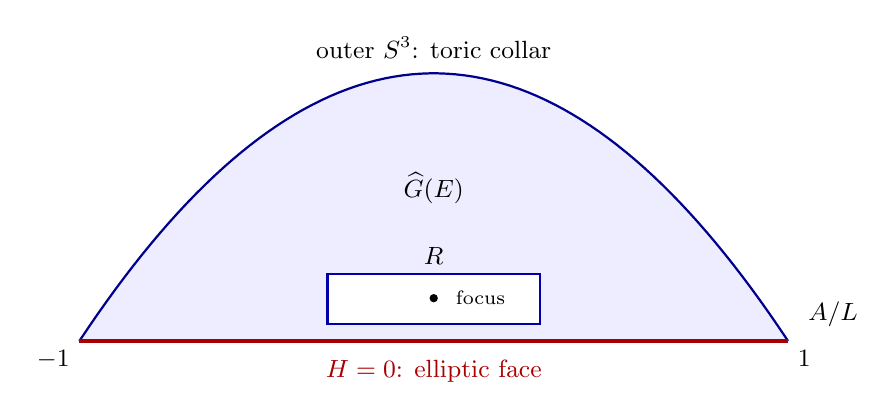
\begin{tikzpicture}[x=4.5cm,y=3.4cm,font=\small]
 \fill[blue!7] (-1,0) -- plot[domain=-1:1,samples=80] (\x,{1-\x*\x}) -- cycle;
 \draw[thick,blue!55!black] plot[domain=-1:1,samples=80] (\x,{1-\x*\x});
 \draw[very thick,red!65!black] (-1,0) -- (1,0);
 \filldraw[fill=white,draw=blue!65!black,thick] (-0.3,0.0625) rectangle (0.3,0.25);
 \fill (0,0.16) circle (1.5pt);
 \node[anchor=west,font=\scriptsize] at (0.035,0.16) {focus};
 \node[anchor=south] at (0,0.25) {$R$};
 \node at (0,0.57) {$\widehat G(E)$};
 \node[anchor=south] at (0,1.02) {outer $S^3$: toric collar};
 \node[anchor=north,text=red!65!black] at (0,-0.035) {$H=0$: elliptic face};
 \node[anchor=north east] at (-1,0) {$-1$};
 \node[anchor=north west] at (1,0) {$1$};
 \node[anchor=west] at (1.03,0.10) {$A/L$};
\end{tikzpicture}
\caption{Normal補完の商座標図．縦座標は $4\pi^2H/L^2$ で，
外側の曲線は $4\pi^2H/L^2=1-(A/L)^2$．白い長方形は固定するfocus blockの像，
淡色部分はnormal exteriorの像である．図は一つの許される寸法の例であり，
integral-affine図ではない．下辺のelliptic faceが大域化の課題として残る．}
\label{ncc:fig:completion-base}
\end{figure}

\begin{corollary}[Closed curveに沿うnormal ball全体への延長]
\label{ncc:product-completion}
定理\ref{tnc:actual-curve}のnormal-trivial symplectic curve $C'$と，
そのproduct neighborhood $C'\times D^4_\rho$を用いる．
既存のconnected-level quotient $q:C'\to\Gamma$に対して，
\[
 \widehat\Pi=(\widehat G,q):C'\times D^4_\rho
              \longrightarrow\Delta_\rho\times\Gamma
\]
は，$C'\times K_c$のfibrationを開近傍ごと保ち，outer normal collarで
標準toric normal fibrationと$q$との積になる．正則fibersはLagrangian $T^3$である．
新たな$H=0$上のwhole fibersは，$\Gamma$のregular point上では$T^2$，
trivalent vertex上では$S^1\times(S^1\vee S^1)$である．
これらはsmooth strata上でisotropicであり，Euler characteristicは零である．
既存のfocus--hyperbolic rank-zero fibersとその個数は変わらない．
\end{corollary}

\begin{proof}
Symplectic product neighborhoodの同型で定理\ref{ncc:normal-ball-completion}の構成を運ぶ．
NormalとcurveのfunctionsはPoisson可換であり，whole fibersは対応するconnected fibersの積である．
Elliptic circleとcurveのcircleまたはfigure-eightの積が表示した新fibersを与える．
それらのEuler characteristicは$\chi(S^1)=0$により零である．
Normal focus fiberとその近傍は変更していないので，focus--hyperbolic fibersは保存される．
\end{proof}

\begin{remark}[Elliptic faceは境界なしの大域化を解決しない]
\label{ncc:elliptic-face-limitation}
この補完はouter normal collarをtoric化するが，$H=0$にgenuineなelliptic base boundaryを作る．
特に$-L<A<L$かつ$\Gamma$のregular point上では，whole elliptic fiberは
normal ballの内部にあるcompact $T^2$で，base germは三次元half-spaceである．
このfiberをwhole fiberとして保ち，その近傍のfiber decompositionも保つ
compact $X_d$ から Hausdorff base への大域quotientは，このbase boundary germを取り除けない．
実際，fiberを含む開集合 $O$ をnormal ballの内部に取る．
大域写像 $p$ はcompact sourceからHausdorff targetへの写像なのでclosedであり，
$B\setminus p(X_d\setminus O)$ はそのfiberの値を含み，全逆像が $O$ に入る開近傍である．
従ってquotient germは元と同じである．
従ってboundary-freeな大域baseを得るには，このelliptic faceの近傍自体を変更するか，
whole fiber条件を変更する追加の構成が必要である．
これはnormal exteriorのfibrationの存在と，大域のboundary-free fillingとを分ける条件である．
\end{remark}

\subsection{Normal exterior の round handle と相対 CW 模型}
\label{tnc:relative-handles-section}

以下で smooth handle の存在と Lagrangian filling の存在を区別する．
$Y=\partial K_c$，$E=D^4\setminus\operatorname{int}K_c$ とし，
outer boundary $S^3=\partial D^4$ を指定する．
Round handle は Asimov \cite{asimov-round} による標準的な道具であるが，
ここで必要な分解は Hopf 商から直接構成する．

\begin{proposition}[Hopf fibers に沿う一つの round handle]
\label{tnc:normal-round-handle}
Corners を丸めた $E$ は，outer $S^3$ を incoming boundary とした
smooth cobordism として，$S^3\times[0,1]$ に
\[
 R=S^1\times D^1\times D^2,
 \qquad \partial_-R=S^1\times\partial D^1\times D^2
\]
を一つ付けて得られる．
二つの attaching solid tori は Hopf fibration $S^3\to S^2$ の
二つの fiber の tubular neighborhoods であり，
その parametrization は円束の局所自明化から取る．
特に core circles は linking number の絶対値が一の Hopf link をなす．
Framing を任意の knot framing に置き換えてよいという主張ではない．

この round handle は通常の $1$-handle と $2$-handle を一つずつに分解できる．
逆向きの cobordism，すなわち $Y$ を incoming とする表示では，
通常の $2$-handle と $3$-handle を一つずつ持つ．
\end{proposition}

\begin{proof}
補題\ref{tnc:focus-exterior-hopf}の商 $B$ は，
solid torus から open $3$-ball を除いたものなので，
outer sphere を incoming として
\[
 B=(S^2\times[0,1])\cup_{\partial D^1\times D^2}(D^1\times D^2)
\]
という smooth relative handle 表示を持つ．
$E\to B$ は principal $S^1$-bundle である．
Sphere collar 上では外側境界の Hopf bundle の積であり，
$D^1\times D^2$ 上では自明である．
従ってこの表示を円束で引き戻すと所要の round handle 表示になる．
Attaching disks の各点の fiber は outer Hopf fiber であり，
二つの core circles は Hopf link である．
円束の局所自明化が全 attaching map を指定するので，
この記述は抽象的な homotopy 型だけによるものではない．

通常の handles への分解も直接見える．
$S^1=I_0\cup I_1$ を端点で交わる二つの閉区間に分ける．
$I_0\times D^1\times D^2$ は core $D^1$，cocore $I_0\times D^2$ を持つ
$4$-dimensional $1$-handle である．
残りの $I_1\times D^1\times D^2$ は core $I_1\times D^1$，cocore $D^2$ を持ち，
\[
 (\partial I_1\times D^1\times D^2)
 \cup(I_1\times\partial D^1\times D^2)
 =\partial(I_1\times D^1)\times D^2
\]
に沿って付く $2$-handle になる．
向きを逆にした handle 表示では index $k$ は $4-k$ になる．
\end{proof}

\begin{lemma}[逆向きの唯一の $2$-handle の attaching class]
\label{tnc:reverse-handle-loop}
命題\ref{tnc:normal-round-handle}の $Y$ から $S^3$ への表示において，
唯一の $2$-handle の attaching loop は，ある $k\in\mathbb Z$ に対して
\[
 a^k b^{\pm1}\in
 \pi_1(Y)=\langle a,b,t\mid[a,b]=[a,t]=1,\ [t,b]=a\rangle
\]
を表す．Whisker と向きを選び直せば，その based class を $b$ とできる．
この一つの関係の normal closure は $a,b$ の両方を殺し，$t$ を残す．
これは attaching loop の homotopy class の主張であり，その knot isotopy class や framing の同定ではない．
\end{lemma}

\begin{proof}
$3$-handle は基本群を変えないので，$\pi_1(Y)\to\pi_1(E)$ の kernel は
唯一の $2$-handle の attaching class の normal closure である．
この class 自身は $\pi_1(E)=\langle\tau\rangle$ で消えるから，
境界写像の表により $a^k b^\ell$ と書ける．
Abelianization では $a$ は零なので，$H_1(E)$ は
$\mathbb Z b\oplus\mathbb Z t$ を関係 $\ell b=0$ で割った群となる．
既知の境界写像では $b$ が零，$t$ が $\mathbb Z$ の生成元へ写るから，
$\ell=\pm1$ でなければならない．
$tbt^{-1}=ab$ による conjugation と loop の向きの反転で $b$ に正規化できる．
$b=1$ は $a=[t,b]=1$ も含意し，残る商は $\mathbb Z t$ である．
\end{proof}

\begin{theorem}[管状補集合を保つ homotopy pushout]
\label{tnc:relative-pushout}
$C=C'$，$V_0=\overline{X_d\setminus\operatorname{int}(C\times D^4)}$ とする．
$p\in S^3$ を固定し，$i:C\to V_0$ を section $z\mapsto(z,p)$ の包含とする．
$W_0=S^1\vee S^2$ の wedge point を $*$ とすると，
$V_0$ からの構造写像を保つ homotopy equivalence
\begin{equation}\label{tnc:eq:relative-pushout}
 \mathcal V\simeq
 V_0\cup_i\bigl(C\times W_0\bigr),
 \qquad (z,*)\sim i(z),
\end{equation}
がある．右辺は homotopy pushout としても解釈できる．
また $i$ は，曲面の標準的な $1$-skeleton を潰す写像
$q:C\to S^2$ と，$e h\in\pi_2(V_0)\simeq\mathbb Z$ を表す写像
$f_e:S^2\to V_0$ の合成に homotopic である．

従って包含 $V_0\to\mathcal V$ は homotopy retraction を持つ．
その homotopy cofiber は
\begin{equation}\label{tnc:eq:relative-cofiber}
 \mathcal V/V_0\simeq
 S^1\vee\bigvee^{2g+1}S^2
 \vee\bigvee^{2g+1}S^3\vee S^4.
\end{equation}
\end{theorem}

\begin{proof}
命題\ref{tnc:focus-exterior-homotopy}の証明中の homotopy pushout 比較は，
outer sphere からの構造写像を保って
\[
 (E,S^3)\simeq(S^3\vee W_0,S^3)
\]
を与える．Cofibration の homotopy extension property を用いれば，
必要な map と homotopies を $S^3$ 上で固定して取れる
\cite[Propositions~0.18--0.19]{hatcher-bct}．
$C$ との積を取り，collar に沿う pushout
$\mathcal V=V_0\cup_{C\times S^3}(C\times E)$ に適用する．
$C\times(S^3\vee W_0)$ は $C\times S^3$ と $C\times W_0$ を
共通の $C$ に沿って貼った空間だから，pushout の結合性から
\eqref{tnc:eq:relative-pushout}を得る．

$V_0$ は simply connected なので，$i$ を曲面の $1$-skeleton 上で
定数となるように homotope できる．この homotopy は曲面全体へ延長できる．
従って変更後の $i$ は $q:C\to S^2$ を通じて分解する．
Hurewicz 同型 $\pi_2(V_0)\simeq H_2(V_0)$ の下で
$i_*[C]=e h$ だから，因子 $S^2\to V_0$ は $f_e$ の homotopy class に属する．
Homotopic attaching map への変更は $V_0$ を固定する homotopy 型を変えない．

右辺では $V_0$ 上の identity と
$C\times W_0\to C\xrightarrow{i}V_0$ を合わせれば retraction になる．
また $V_0$ を潰すと
\[
 (C\times W_0)/(C\times\{*\})
 = C_+\wedge W_0
 \simeq (S^1\vee\Sigma C)\vee(S^2\vee\Sigma^2C)
\]
である．ここで $C_+$ は disjoint basepoint を加えた空間である．
例えば $C_+\wedge S^1$ は $C\times I$ の両端を一つの点に潰した空間で，
$C$ の基点を通る区間を選ぶと $S^1\vee\Sigma C$ に分裂する．
さらに一回 suspend すれば $S^2\vee\Sigma^2C$ を得る．
曲面の $2$-cell の attaching word は commutators の積であり，
その suspension は各 $S^2$ 成分への degree が零だから null-homotopic である．
従って $\Sigma C\simeq\bigvee^{2g}S^2\vee S^3$ であり，
式\eqref{tnc:eq:relative-cofiber}が従う．
\end{proof}

\begin{proposition}[六次元の相対 handle 数と次数関係]
\label{tnc:product-relative-handles}
$W=C\times E$ とし，
$A_{\mathrm{out}}=C\times S^3$，$A_{\mathrm{in}}=C\times Y$ とする．
$W$ は $A_{\mathrm{out}}$ から，通常の smooth handles を
\[
\begin{array}{c|rrrr}
 \text{index}&1&2&3&4\\ \hline
 \text{個数}&1&2g+1&2g+1&1
\end{array}
\]
だけ付けて得られる．これらの個数は各次数の相対整数 Betti 数に等しい．
特にどの smooth relative handle 表示でも index $4$ の handle は少なくとも一つ必要である．

式\eqref{tnc:eq:relative-pushout}で $i=f_e q$ に正規化した相対 CW 模型では，
$C$ の $2$-cell と $S^1$ の $1$-cell の積から来る $3$-cell が，
次数二の equivariant 関係
\[
 e(\tau-1)h=0
\]
を与える．これは smooth attaching sphere の isotopy class や framing を決定する主張ではない．
\end{proposition}

\begin{proof}
命題\ref{tnc:normal-round-handle}による $E$ の relative Morse function は
index $1,2$ の critical points を一つずつ持つ．
$C$ との積では，これら二点に対応する critical submanifolds は $C$ である．
$C$ 上の，index $0,1,2$ の critical points がそれぞれ $1,2g,1$ 個の Morse function を用いて，
各 critical submanifold の近傍で十分小さい Morse--Bott perturbation を行う．
境界 collar 上では元の関数を保ち，critical locus の外では微分が零から離れているので，
小さい perturbation は新しい critical points を生じない．
Index は和になるため表示した個数を得る．

Pair $(E,S^3)$ の相対 homology は次数 $1,2$ でそれぞれ $\mathbb Z$，
他の次数では零である．K\"unneth 公式により
\begin{equation}\label{tnc:eq:relative-homology-out}
 H_k(W,A_{\mathrm{out}};\mathbb Z)\simeq
 \begin{cases}
  \mathbb Z,&k=1,4,\\
  \mathbb Z^{2g+1},&k=2,3,\\
  0,&\text{その他}.
 \end{cases}
\end{equation}
相対 cellular chain group の rank は同じ次数の homology rank 以上なので，
各 handle 個数はこの homological lower bound を達成している．
Excision により同じ相対群は $H_k(\mathcal V,V_0;\mathbb Z)$ でもある．

最後の関係は，正規化した $i=f_eq$ に対する product CW construction から読める．
曲面の $1$-cells は $V_0$ 内で定数であり，
それらと $S^1$ の積は $2g$ 個の新しい $2$-cells を与える．
曲面の $2$-cell と $S^1$ の積の boundary で，$S^1$ 方向の両端は
universal cover の隣接する二つの $V_0$ に入り，それぞれ $\tau e h$ と $e h$ を表す．
残る側面は曲面の commutator word に沿う．
その各 $1$-cell は正負に一回ずつ現れ，曲線方向の loops は deck group へ自明に写るので，
新しい $2$-cells に対する係数は全て零である．
従って向きを選べば境界は $e(\tau-1)h$ になる．
ここで述べているのは，$V_0$ 内部の関係を既に課した次数二の module 上の表示である．
この計算だけから，smooth handles の framed attaching maps 全体や
$4$-cell の attaching map を推定しない．
\end{proof}

\begin{corollary}[Weinstein cobordism による全体移行の障害]
\label{tnc:no-weinstein-normal-transition}
$W=C\times E$ は，$A_{\mathrm{out}}$ と $A_{\mathrm{in}}$ を二つの全境界成分として，
どちらを incoming boundary としても Weinstein cobordism にはならない．
これは任意の候補 Weinstein structure に対する位相的な障害である．
\end{corollary}

\begin{proof}
実六次元の Weinstein cobordism の Morse handles は index $3$ 以下である．
実際，Liouville vector field の stable manifolds は isotropic なので，
Morse index は複素次元以下になる
\cite[Section~1]{cieliebak-eliashberg-flexible-local}．
従って incoming boundary に対する次数 $3$ より上の相対 homology は零でなければならない．
$A_{\mathrm{out}}$ が incoming なら，式\eqref{tnc:eq:relative-homology-out}の
$H_4(W,A_{\mathrm{out}})=\mathbb Z$ がこれに反する．
逆向きでは Poincar\'e--Lefschetz duality と相対群の torsion-freeness により
\[
 H_5(W,A_{\mathrm{in}};\mathbb Z)
 \simeq H^1(W,A_{\mathrm{out}};\mathbb Z)=\mathbb Z
\]
であり，やはり不可能である．
\end{proof}

\begin{remark}[障害の範囲]
\label{tnc:relative-handles-scope}
上の否定は，二つの閉境界成分をそのまま incoming/outgoing として扱う
Weinstein cobordism に対するものである．
Boundary を切り分けて新しい側面を加える場合，
非 exact な symplectic cobordism，あるいは singular Lagrangian fibration の存在は否定しない．
特に smooth handle 表示は得られたが，それを Weinstein handles だけで実現して
normal face を埋める方法は採用できない．
また cofiber の wedge 分解から $\mathcal V$ 自体を
$V_0$ とその cofiber の wedge と同一視してはいけない．
その誤同定は $e(\tau-1)h$ の関係を失う．
\end{remark}


\begin{corollary}[曲線を切った場合の相対 homology]
\label{tnc:punctured-relative-handles}
$C^\circ$ が genus $g$，$r\ge1$ 個の境界成分を持つ compact surface なら，
\[
 H_k(C^\circ\times E,C^\circ\times S^3;\mathbb Z)
 \simeq
 \begin{cases}
  \mathbb Z,&k=1,\\
  \mathbb Z^{2g+r},&k=2,\\
  \mathbb Z^{2g+r-1},&k=3,\\
  0,&\text{その他}.
 \end{cases}
\]
従って outer boundary に対する次数 $4$ の障害は消えるが，
新しい側面 $\partial C^\circ\times E$ の接続条件が生じる．
Weinstein structure の存在をこの消滅から結論しない．
\end{corollary}
\begin{proof}
$C^\circ$ の homology は $H_0=\mathbb Z$，
$H_1=\mathbb Z^{2g+r-1}$ のみなので，
$(E,S^3)$ の相対 homology との K\"unneth 公式が表示を与える．
ここで relative subspace は $C^\circ\times S^3$ だけであり，
$\partial C^\circ\times E$ を incoming boundary に含めた計算ではない．
\end{proof}

\subsection{境界を埋める円板の非可換関係}
\label{tnc:relative-disk-extension}

境界包含の基本群写像の kernel を求めるだけでは，
各 loop を埋める円板の間に必要な関係は分からない．
ここでは normal pair の crossed module と，三次元補集合の
第二相対 homotopy group の通常の群構造を計算する．
三次元全体での全境界作用の表示，smooth handle の framing，
isotropic attaching sphere の構成までは結論しない．

\begin{theorem}[Normal pair の相対円板と二階差分]
\label{tnc:normal-relative-disk-module}
$Y\hookrightarrow E$ の relative group は abelian であり，
$\pi_1(Y)$ の作用は $\pi_1(E)=\langle\tau\rangle$ を経由する．
従って $\mathfrak R_E=\pi_2(E,Y)$ は $\Lambda$-module となる．
逆向きの唯一の $2$-handle の core に，適切な向きと whisker を与え，
その boundary が $b$ となる relative disk class $B$ を選べば
\[
 \mathfrak R_E\simeq\Lambda B
\]
とできる．$\langle a,b\rangle\simeq\mathbb Z^2$ をこの式でだけ加法的に書けば，
boundary は Laurent polynomial $f$ に対して
\[
 \partial(fB)=f(1)b+f'(1)a
\]
である．従って $\pi_2(E)$ の適当な $\Lambda$-generator
$\nu_{\mathrm{rel}}$ に関して exact sequence
\[
 0\longrightarrow\Lambda\nu_{\mathrm{rel}}
   \xrightarrow{\ \nu_{\mathrm{rel}}\mapsto(\tau-1)^2B\ }
   \Lambda B\xrightarrow{\partial}\mathbb Z a\oplus\mathbb Z b
   \longrightarrow0
\]
を得る．以下では $\pi_2(E)$ をその像と同一視する．$A=(\tau-1)B$ と置くと
\[
 \partial A=a,\qquad
 {}^tB=B+A,\qquad {}^tA=A+\nu_{\mathrm{rel}}.
\]
$\nu_{\mathrm{rel}}$ と既存の sphere generator の差は
$\pm\tau^n$ という unit の選択だけであり，marked torus の向きを
暗黙に固定し直しているわけではない．
\end{theorem}
\begin{proof}
$Y$ の universal cover は contractible である．
従って pair の homotopy 長完全列と
$\pi_1(Y)\to\pi_1(E)$ の計算により
\[
 1\longrightarrow\pi_2(E)\longrightarrow\mathfrak R_E
   \longrightarrow\langle a,b\rangle\longrightarrow1
\]
となり，kernel は crossed-module の Peiffer identity により central である．
$\widehat Y\subset\widetilde E$ を connected inverse image とすると，
$\widehat Y\cong T^2\times\mathbb R$ である．
この central extension の class は，次の証明でも詳述する
homotopy-fiber の記述により
\[
 H_2(\widehat Y;\mathbb Z)\longrightarrow
 H_2(\widetilde E;\mathbb Z)=\pi_2(E)
\]
で決まる．この写像は零である．実際，generator $F$ は
補題\ref{tnc:normal-boundary-maps}の $S^1_a\times D^2_b$ で埋まり，
その solid torus の基本群の $\pi_1(E)$ への像が零なので，
solid torus 全体が $\widetilde E$ へ持ち上がる．
$H_1(T^2;\mathbb Z)$ は free なので extension class に他の成分はない．
よって extension は abelian groups の direct product として split し，
$\mathfrak R_E$ は abelian である．

境界の kernel $\langle a,b\rangle$ の作用は，その relative lift による
inner conjugation に等しいから trivial である．従って全境界作用は
$\langle\tau\rangle$ を経由する．また
$(\widetilde E,\widehat Y)$ は $1$-connected pair である．
一般の relative Hurewicz theorem は
$\pi_1(\widehat Y)$ の作用による quotient を取って初めて成立するが
\cite[Theorem~4.37]{hatcher-bct}，ここでは今述べた作用が trivial なので
\[
 \mathfrak R_E\simeq H_2(\widetilde E,\widehat Y;\mathbb Z)
\]
を $\Lambda$-module として得る．

命題\ref{tnc:normal-round-handle}の reversed relative handle decomposition は
一つの index-$2$ handle と一つの index-$3$ handle からなる．
従って universal-cover relative cellular chain は，次数 $2,3$ に
それぞれ一つの $\Lambda$ を持ち，他の次数では零である．
上の exact sequence の quotient $\mathbb Z^2$ は
$(\tau-1)^2$ で殺されるので，$\mathfrak R_E$ の $\Lambda$-rank は一である．
もし唯一の differential $d_3:\Lambda\to\Lambda$ が非零なら，
$\Lambda$ の fraction field 上で同型となり，この rank は零になってしまう．
従って $d_3=0$ であり，$\mathfrak R_E\simeq\Lambda$ である．
補題\ref{tnc:reverse-handle-loop}により，index-$2$ handle の orientation と
whisker を選んで，その disk class $B$ の boundary を $b$ にできる．
これは relative cellular generator なので $\Lambda$-basis となる．

$\pi_1(Y)$ の relation $tbt^{-1}=ab$ から
$\partial(\tau^nB)=b+n a$ が全ての $n\in\mathbb Z$ に対して成立する．
これが $\partial(fB)=f(1)b+f'(1)a$ を与える．
その kernel は $f(1)=f'(1)=0$，すなわち
$(\tau-1)^2\Lambda$ である．$\pi_2(E)\simeq\Lambda$ の generator を
unit 倍して $\nu_{\mathrm{rel}}\mapsto(\tau-1)^2B$ とすれば，
残りの式は $A=(\tau-1)B$ から従う．
\end{proof}

\begin{remark}[Normal disk action の意味]
$a$ と $b$ は $E$ の中でともに null-homotopic であるが，
その filling disks を $t$ に沿って運ぶ操作は自明ではない．
一度の差分が $a$ の disk を作り，二度の差分が sphere generator を作る．
これは normal pair の crossed module を決定する計算であり，
円板が Lagrangian であることや，handle framing が symplectic attachment に
適合することを追加で主張しない．
\end{remark}

$\mathcal A=\partial\mathcal U=C\times Y$，
$\Gamma_C=\pi_1(C)$ とし，
\[
 M=\pi_2(\mathcal V),\qquad
 \mathfrak R=\pi_2(\mathcal V,\mathcal A).
\]
$M$ は定理\ref{tnc:equivariant-pi2}で求めた $\Lambda$-module であるが，
次の central extension ではその underlying abelian group を使う．
$h\in M$ は一つの $V_0$ の lift の正の二次元生成元とする．

\begin{theorem}[Relative disk group の central extension]
\label{tnc:relative-disk-central-extension}
境界写像によって exact sequence
\[
 1\longrightarrow M\xrightarrow{\iota}\mathfrak R
   \xrightarrow{\partial}\Gamma_C\times\mathbb Z_a\times\mathbb Z_b
   \longrightarrow1
\]
を得る．$\iota(M)$ は $\mathfrak R$ の中心に含まれる．
Surface generators $\alpha_i,\beta_i$ ($1\le i\le g$) と向きを固定し，
その相対円板による lifts を $A_i,B_i$，$a,b$ の lifts を
$\mathfrak a,\mathfrak b$ とする．符号規約を曲線の向きに合わせると，
この extension は
\[
 \prod_{i=1}^g[A_i,B_i]=\iota(eh)
\]
および $\iota(M)$ の centrality と
\[
 [\mathfrak a,\mathfrak b]=1,\qquad
 [\mathfrak a,A_i]=[\mathfrak a,B_i]
 =[\mathfrak b,A_i]=[\mathfrak b,B_i]=1
\]
を relations として表示される．ここで $M$ 自身の全加法的関係を
$\iota(m+n)=\iota(m)\iota(n)$ として含める．
この central extension は split しない．
\end{theorem}

\begin{proof}
$C$ は genus $g\ge3$ の閉曲面，$Y$ は $T^2$ の mapping torus なので，
$\mathcal A$ は aspherical である．
定理\ref{tnc:actual-complement-pi1}により
\[
 K:=\ker\bigl(\pi_1(\mathcal A)\to\pi_1(\mathcal V)\bigr)
   =\Gamma_C\times\langle a,b\rangle
   \simeq\Gamma_C\times\mathbb Z^2.
\]
$\pi_2(\mathcal A)=0$ と pair の homotopy 長完全列から，
主張した short exact sequence を得る．
相対境界 $\partial:\pi_2(\mathcal V,\mathcal A)\to\pi_1(\mathcal A)$
は fundamental crossed module である
\cite[Section~2]{brown-relative-pi2}．
Peiffer identity において $\partial\iota(m)=1$ と置けば，
$\iota(m)$ と全ての相対類との可換性が従う．

$\widehat{\mathcal A}\to\mathcal A$ を $K$ に対応する connected cover とする．
$Y$ の mapping-torus base を $\mathbb R$ に持ち上げる被覆なので
\[
 \widehat{\mathcal A}\cong C\times T^2\times\mathbb R.
\]
これは universal cover $\widetilde{\mathcal V}$ の境界の逆像である．
Relative disks とその homotopies の一意的 lift により
\[
 \pi_2(\mathcal V,\mathcal A)
   \simeq\pi_2(\widetilde{\mathcal V},\widehat{\mathcal A}).
\]

この central extension の class は
\[
 H^2(K;M)=H^2(C\times T^2;M)
   \simeq\operatorname{Hom}\bigl(H_2(C\times T^2;\mathbb Z),M\bigr)
\]
に属する．最後の同型は $H_1(C\times T^2;\mathbb Z)$ が free であることと
universal coefficient theorem による．
ここで $K$ の coefficient $M$ への作用は trivial であり，
full boundary group の作用が trivial だという意味ではない．
Central extensions の $H^2$ による分類は
\cite[Section~2]{conrad-group-extensions}を参照．

この class が，inclusion による写像
\[
 H_2(\widehat{\mathcal A};\mathbb Z)
   \longrightarrow H_2(\widetilde{\mathcal V};\mathbb Z)=M
\]
そのものであることも確認しておく．
$\widetilde{\mathcal V}$ は simply connected なので，
$H^2(\widetilde{\mathcal V};M)$ の identity に対応する class を
代表する map $p:\widetilde{\mathcal V}\to K(M,2)$ がある
\cite[Theorem~4.57]{hatcher-bct}．
$p$ は $\pi_2$ 上で identity を誘導する．
Inclusion $j:\widehat{\mathcal A}\to\widetilde{\mathcal V}$ と
$p j$ の homotopy fibers の $\pi_1$ は，homotopy 長完全列の比較により
kernel $M$ と quotient $K$ を保って同型になる．
後者は $p j$ が表す $H^2(K;M)$ の class に対応する central extension である．
実際，one-skeleton の lifts を選び，two-cell の境界を一周すると，
$p j$ のその two-cell 上の値が central な relation として現れる．
従って extension class の evaluation は上の inclusion map と一致する．

その写像を K\"unneth 分解で計算する．
$[C]\times\{*\}$ は $e h$ へ写る．
$H_1(C)\otimes H_1(T^2)$ は inclusion が
$C\times\widetilde E$ を経由し，$H_1(\widetilde E)=0$ なので零へ写る．
最後の $[T^2]=F$ も零へ写る．
これには ordinary $H_2(E)$ への消滅だけでは足りないが，
補題\ref{tnc:normal-boundary-maps}の explicit solid torus
$S^1_a\times D^2_b\subset E$ は，その $\pi_1$ が $\pi_1(E)$ で零となるため
$\widetilde E$ に持ち上がり，lift した $F$ を埋める．
ゆえに extension class は surface orientation class $u_C$ を用いて
\[
 (e h)\,\operatorname{pr}_C^*u_C
\]
である．Surface polygon の relation と全ての mixed tori に評価すれば，
上の presentation を得る．

最後に ambient hyperplane class による homomorphism
\[
 \ell:M\longrightarrow\mathbb Z,\qquad
 \ell(m)=\langle H,m\rangle
\]
は $\ell(h)=1$ を満たす．特に $e h\ne0$ なので extension class は非零であり，
extension は split しない．
\end{proof}

\begin{corollary}[Curve relation の不変性と degree の quotient]
\label{tnc:relative-disk-degree}
Curve generators を埋める相対円板を選び直しても，
$\prod_i[A_i,B_i]=\iota(e h)$ は変わらない．
さらに normal base circuit $t$ の作用との整合性は
$e(\tau-1)h=0$ を要求する．
また $\ell$ を上の homomorphism とすると，
\[
 \mathfrak R/\iota(\ker\ell)
   \simeq\pi_1(P_e)\times\mathbb Z^2,
\]
ただし $P_e\to C$ は Euler number $e$ の oriented circle bundle
（boundary orientation の規約に応じて全体の符号を固定）である．
\end{corollary}
\begin{proof}
同じ boundary loop の二つの lifts の差は central subgroup $\iota(M)$ に属する．
従って各 commutator は不変である．
$t$ は $\pi_1(\mathcal A)=\Gamma_C\times\pi_1(Y)$ の中で
curve generators と可換なので，$t$ を作用させた $A_i,B_i$ も同じ
curve generators の lifts である．左辺は変わらず，右辺は
$\iota(e\tau h)$ へ写るため $e\tau h=e h$ を得る．
最後の quotient は，central subgroup $M$ を $\ell$ によって
$\mathbb Z\langle z\rangle$ へ押し出した extension である．
その presentation は
\[
 \prod_i[A_i,B_i]=z^e,
 \qquad z\ \text{central},
\]
と独立な二つの central generators $\mathfrak a,\mathfrak b$ からなる．
Surface polygon の clutching degree $e$ による circle bundle の
fundamental group と一致する．
\end{proof}

\begin{remark}[相対円板計算の範囲]
これは boundary loops が個々に消えるという条件を，
その filling disks が満たすべき nonabelian relation へ強めたものである．
Curve relation を全て自明にする disk system は存在しない．
ただし，$t$ による各 disk lift の作用の全表示，embedded disk の選択，
smooth handle framing，Lagrangian attaching data はまだ決定していない．
また $\mathcal A$ 自体は Lagrangian ではないから，
$\mathfrak R$ 全体に symplectic area を relative homotopy invariant として
定義してはならない．Sphere subgroup $M$ 上では
$\int_m\omega=a\ell(m)$，$\langle c_1(TX_d),m\rangle=(5-d)\ell(m)$
であり，この sphere ambiguity と boundary action periods は区別する．
\end{remark}

\subsection{Marked cycleのMaslov classとclean Lagrangian disk}
\label{ncc:maslov-clean-disk-section}

\begin{lemma}[Normal regular torusのMaslov marking]
\label{ncc:normal-maslov-marking}
元の模型$G_c$のregular torus $L_{A,q}$で，$a$をinverse-phase circle，
$b$を$w-c$のpositive phaseを一周する任意のsection liftとする．
標準trivialization $\Omega=dX\wedge dY$に関するMaslov classは
\[
 \mu_L(a)=0,\qquad \mu_L(b)=2.
\]
従って$L_{A,q}$と境界でcleanに交わるsmooth embedded Lagrangian diskが
$\mathbb C^2$内に存在するなら，その境界のclass $ma+nb$は$n=0$を満たす．
さらに標準primitiveに対するStokesの定理により$mA=0$である．
特にprimitiveなessential境界classなら$A=0$かつ$\partial D=\pm a$でなければならない．
\end{lemma}

\begin{proof}
周期一のgeneratorを$V_a=2\pi(iX,-iY)$と書く．Torusのもう一つのtangent vectorを$v$とすると
\[
 \Omega(V_a,v)=2\pi i\,dw(v).
\]
$w=c+\sqrt q\,e^{i\theta}$に沿って$v$を選べば，右辺のphaseは$\theta$が一周すると一回転する．
$a$に沿っては$w$とこのphaseは変化しない．Squared phaseのwindingを取るMaslov規約により
最初の二つの式が従う．Section liftの変更は$b$へ$a$の整数倍を加えるだけなので結果は変わらない．

一般に，二つのLagrangian surfaces $L,D$がsmooth boundary curve $\gamma=\partial D$に沿って
cleanに交わるとする．その共通tangent lineを$\ell=T\gamma$とおく．
Symplectic plane bundle $\ell^\omega/\ell$内で，二つのtangent planesの商は互いに異なるreal linesである．
その相対角は$\mathbb R/\pi\mathbb Z$の一点を除いたintervalに値を取るので，
両tangent-plane loopsのsquared phasesはhomotopicである．$D$のphaseはdisk全体へ延びるため，
$\mu_L(\gamma)=0$となる．これを上の計算と合わせれば$n=0$を得る．

標準primitive
\[
 \lambda_0=\tfrac12\operatorname{Im}(\overline X\,dX+\overline Y\,dY)
\]
は$\int_a\lambda_0=A$を満たす．Lagrangian diskには$\omega_0|_D=0$なので
\[
 0=\int_D\omega_0=\int_{\partial D}\lambda_0=mA
\]
である．Primitiveなessential classで$n=0$なら$m=\pm1$であり，結論を得る．
\end{proof}

\begin{remark}
この障害は，null-homotopicなmarked loopをclean Lagrangian core diskで埋める方法への制約である．
Elliptic degenerationでcircleを潰すときのtransverse diskはsymplecticであり，この障害の対象ではない．
従って上のnormal completionと矛盾しない．また，diskがcurve方向にも動く三次元ambientの場合や，
boundaryでclean条件を失うsingular diskへの非存在をここでは主張しない．
\end{remark}
